\section{Обсуждение}\label{sec:disc}

\cref{tab:cbms_tab} демонстрирует превосходство Sparse-CBM по сравнению с Label-free на всех наборах данных, кроме ImageNet и Places365. Более того, Contrastive-CBM имеет самый низкий общий балл. Мы интерпретируем эти наблюдения следующим образом:

\begin{figure}[t]
\begin{center}
\centerline{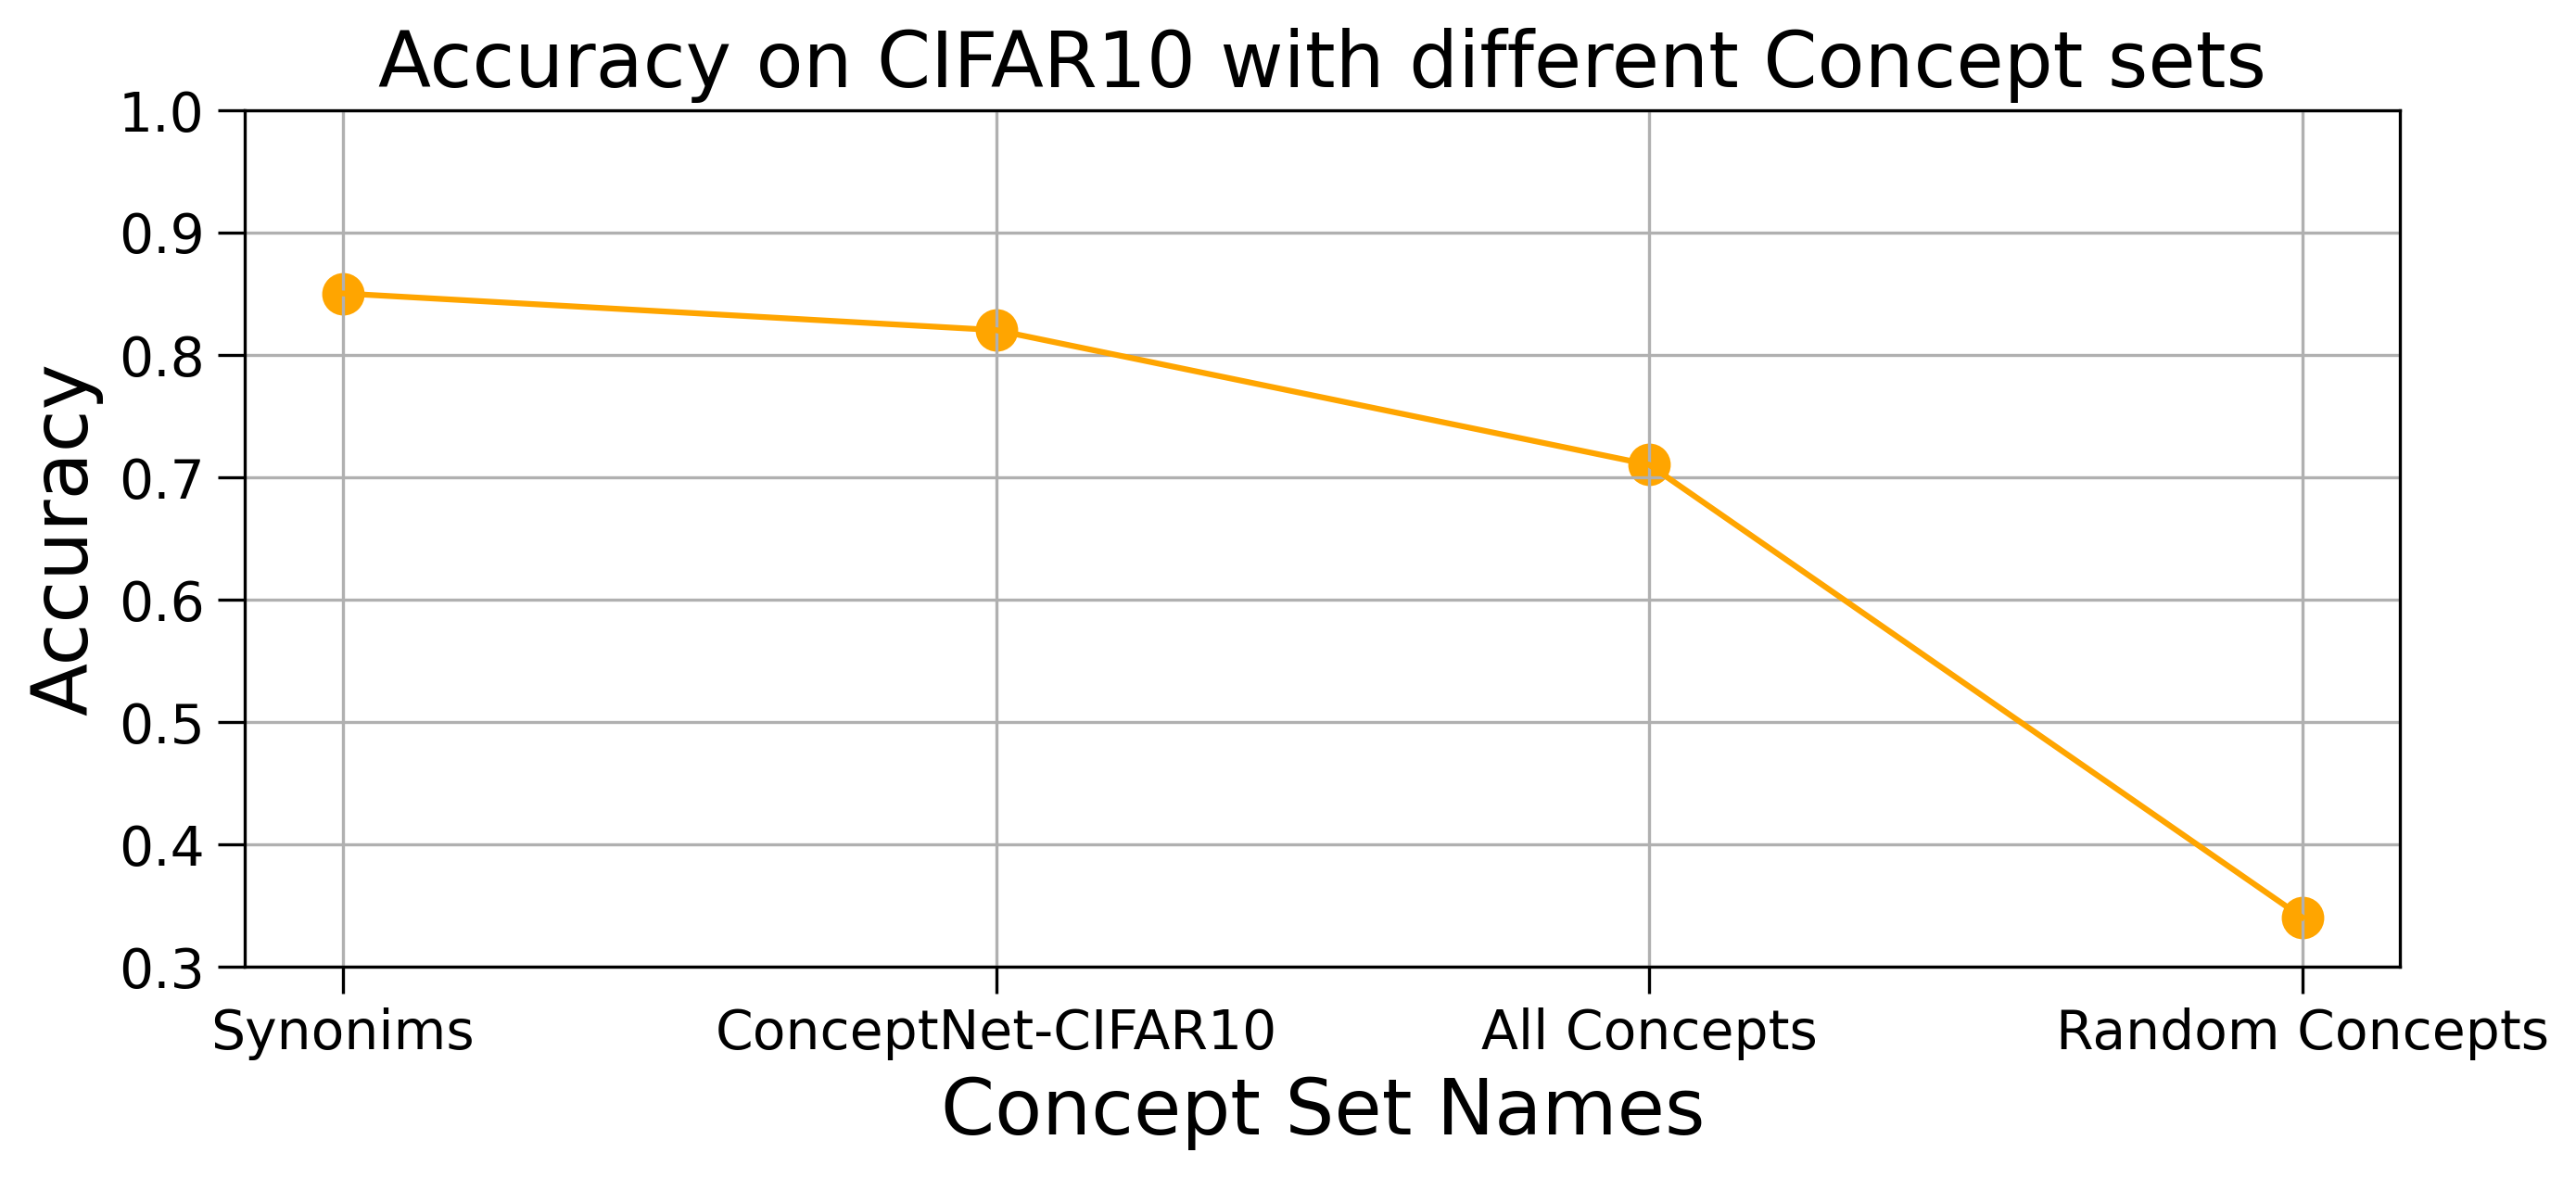
\includegraphics[width=\columnwidth]{./figures/cms_acc_cifar10.png}}
\caption{Зависимость качества CMS от набора конйептов.}
\label{fig:cms_acc}
\end{center}
\end{figure}



1) Из-за \cref{tab:concepts_size} пропорция между размером CBL и размером FC различается. В то время как такие наборы данных, как CIFAR10 и CIFAR100, содержат в $\approx$ 10 раз больше концептов, чем классов, для ImageNet и Places365 это число, а значит и пропорция между размерами слоев, примерно в 4,6-4,7 раза больше. Мы настаиваем на том, что разреженность внутренних слоев приносит больше пользы при увеличении размерности CBL по сравнению с размерностью выхода последнего полностью связанного слоя.

2) Методу Contrastive-CBM не хватает интерпретируемости представления концептов, т. е. разреженности CBL (подробное сравнение интерпретируемости см. в \cref{sec:concepts_interpretability}).

Мы также ссылаемся на алгоритм CMS и показываем снижение точности в зависимости от "качества" концептов, что делает наш метод и подобные ему менее универсальными. С другой стороны, при "хорошем" наборе понятий для каждого набора данных мы показываем, что CMS превосходит Zero-shot CLIP. Это говорит о том, что модель получает дополнительную "уверенность" при предсказании не только наиболее похожего класса, но и при получении нескольких значимых концептов на изображение.

\subsection{Исследование абляции}\label{sec:abl}
Компоненты, введенные в наш фреймворк, приводят к снижению итоговой производительности по сравнению с линейным зондированием (см. \cref{tab:cbms_tab}), обеспечивая при этом интерпретируемость, которую мы представляем в \cref{sec:concepts_interpretability}. Наш метод и его интуиция, заключающаяся в том, чтобы сделать внутреннее представление более разреженным, понятны, и он оказывается перспективным для извлечения значимых понятий. Тем не менее, "жесткая" (т.е. делающая выборки непосредственно одномоментными) выборка в контрастном Gumbel-Softmax loss скорее вредит производительности Sparse-CBM, чем улучшает ее. В то же время Contrastive-CBM выполняет двойной softmax на CBL, который обеспечивает отсутствие разреженности и достигает худшего результата по точности, что опять же подтверждает нашу гипотезу о полезности разреженных внутренних представлений. И фреймворк CBM, и метод CMS полагаются на сгенерированный набор концептов. С концептами, которые лучше приспособлены к набору данных, мы показываем более высокие результаты по точности классификации, с другой стороны, мы хотим, чтобы концепты были более разнообразными, что эмпирически определено в \cref{sec:framework} и в предыдущей \cite{oikarinen2023labelfree} работе, тогда нам не принципиально менять количество концептов вручную, мы предпочтем сохранить сгенерированные.

\subsection{Ограничения}\label{sec:lims}

Помимо достигнутых показателей точности, мы сообщаем об основных ограничениях нашего фреймворка и алгоритма \ref{Alg:CMS}. LLM, предложенный во фреймворке CBM, по-прежнему не влияет на процесс классификации, то есть не поддерживает генерацию концептов во времени и работает только на \textbf{шаге 2}. Оба варианта CMS и CBM не модифицируют латентное пространство CLIP, что делает наш подход менее универсальным. Хотя мы вносим вклад в понимание разреженных CBL, эффективность моделей узких мест с также разреженными FC все еще не раскрыта. То же самое относится и к проблеме сквозного редактирования концепт-блотлека (см. \cref{sec:bottls}). Наконец, метод CMS может быть полезен в качестве дополнения к CLIP, но в долгосрочной перспективе не может конкурировать с подходами МД из-за ситуации, показанной в \cref{fig:cms_acc}.   
\nocite{JMLR:v9:vandermaaten08a}